\documentclass[tikz,border=6pt]{standalone}
\usepackage{pgfplots}
\usepgfplotslibrary{groupplots}
\usetikzlibrary{calc}
\pgfplotsset{compat=1.18}
\begin{document}
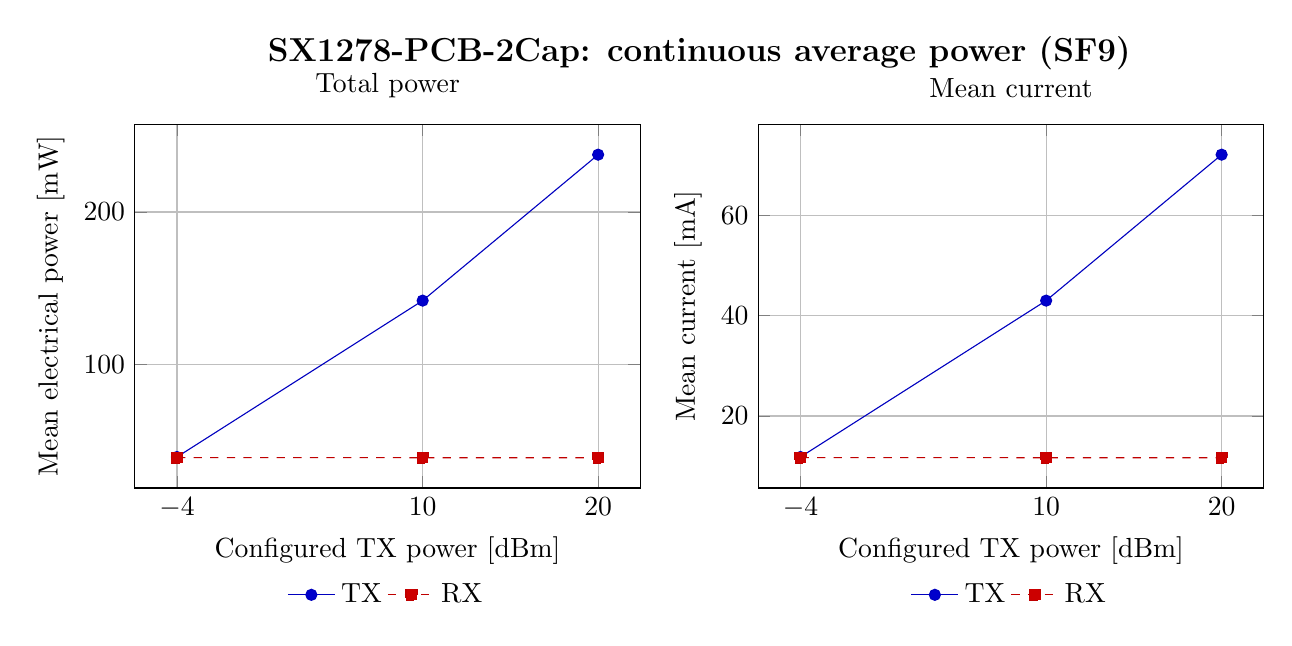
\begin{tikzpicture}
\begin{groupplot}[group style={group size=2 by 1,horizontal sep=1.5cm},width=8cm,height=6.2cm,xtick={-4,10,20},xlabel={Configured TX power [dBm]},grid=both,legend style={draw=none,at={(0.5,-0.23)},anchor=north,legend columns=2}]
\nextgroupplot[title={Total power},ylabel={Mean electrical power [mW]}]
\addplot+[blue!75!black,mark=*] coordinates {(-4,39.0509973) (10,141.803079) (20,237.698424)};\addlegendentry{TX}
\addplot+[red!75!black,dashed,mark=square*] coordinates {(-4,38.651089) (10,38.5895556) (20,38.5792213)};\addlegendentry{RX}
\nextgroupplot[title={Mean current},ylabel={Mean current [mA]}]
\addplot+[blue!75!black,mark=*] coordinates {(-4,11.8336355) (10,42.9706299) (20,72.0298254)};\addlegendentry{TX}
\addplot+[red!75!black,dashed,mark=square*] coordinates {(-4,11.7124512) (10,11.6938047) (20,11.6906731)};\addlegendentry{RX}
\end{groupplot}
\node[font=\bfseries\large] at ($(group c1r1.north)!0.5!(group c2r1.north)+(0,0.9cm)$) {SX1278-PCB-2Cap: continuous average power (SF9)};
\end{tikzpicture}
\end{document}
